\chapter{Results and Discussion}
\label{ch:results}
Currently the graphite database contains 1213 data element. In the plot below each data element is the leaf in the directory tree represented by a file icon. This plot for one the psuedorange and standard deviation from the \ac{gps} receiver. Each data element contains a data point for each second of the day, 86400 points.  This is just a first cut at getting data loaded into the system, but the design will support many data elements and calculations done between elements.
\\ \\
\resizebox{\columnwidth}{!}{
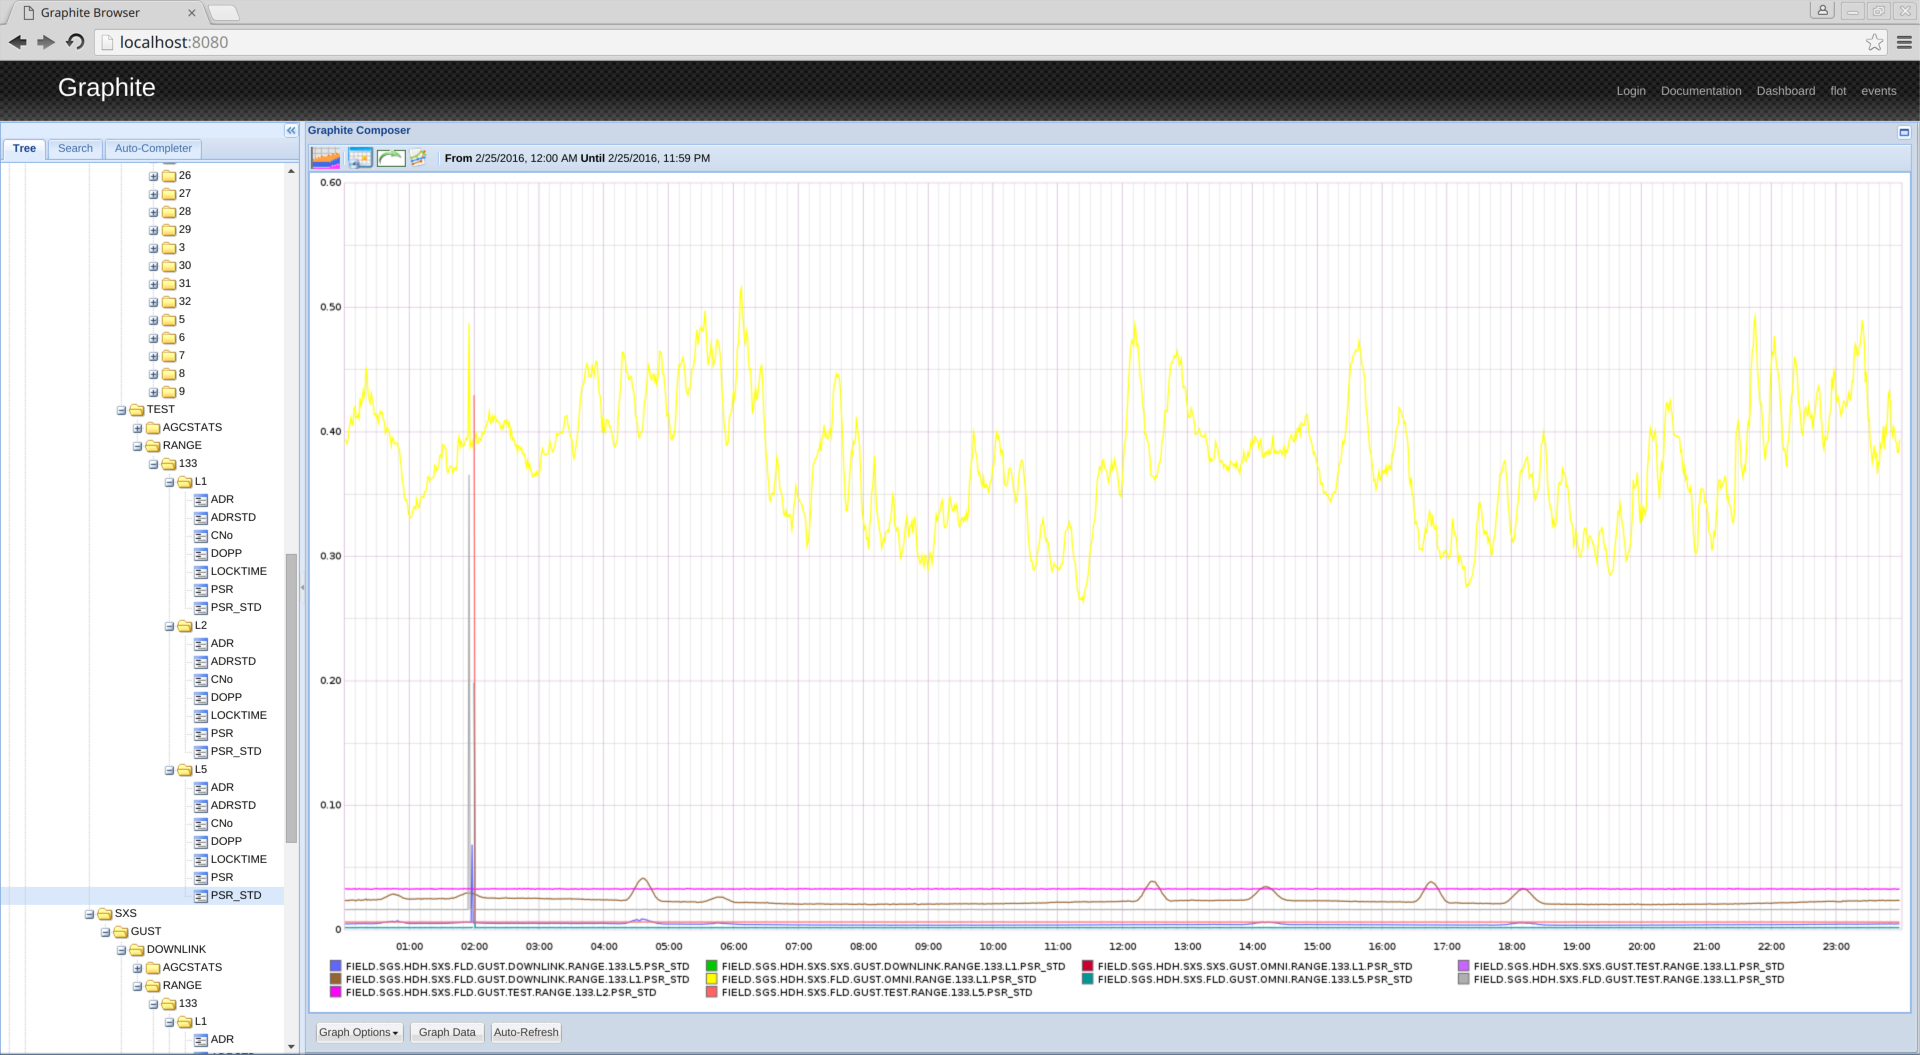
\includegraphics[scale=.25]{figures/PSR_STD-2016-02-25}
}
